\begin{problem}[1]
  Use cylindrical and spherical coordinates to find the volume of a sphere with
  radius $a$.
\end{problem}

\begin{proof}[Solution]
  Graphing the sphere $x^2 + y^2 + z^2 = a^2$ gives us the following
  \begin{multicols}{2}
    \begin{figure}[H]
      \centering
      \includegraphics[width=0.4\textwidth]{./image-files/homework-04/problem-01-solid.jpg}
      \caption{Sphere $x^2 + y^2 + z^2 = a^2$}
      \label{fig:solid_1}
    \end{figure}
    \columnbreak
    Cylindrical coordinates: Converting the sphere $x^2 + y^2 + z^2 = a^2$ to
    cylindrical coordinates gives $r^2 + z^2 = a^2$ and solving for $z$ gives us
    $z = \sqrt{a^2 - r^2}$. The volume element in cylindrical coordinates is
    $\dd{V} = r \dz\, \,\dr \,\dd{\theta}$. The bounds for $\theta$ are $0 \le
    \theta \le 2\pi$, the bounds for $r$ are $0 \le r \le a$, and the bounds for
    $z$ are $-\sqrt{a^2 - r^2} \le z \le \sqrt{a^2 - r^2}$.

    Spherical coordinates: Converting the sphere $x^2 + y^2 + z^2 = a^2$ to
    spherical coordinates gives $\rho^2 = a^2$ and solving for $\rho$ gives us
    $\rho = a$. The volume element in spherical coordinates is $\dd{V} = \rho^2
    \sin(\phi) \,\dd{\rho} \,\dd{\phi} \,\dd{\theta}$. The bounds for $\rho$ are
    $0 \le \rho \le a$, the bounds for $\phi$ are $0 \le \phi \le \pi$, and the
    bounds for $\theta$ are $0 \le \theta \le 2\pi$.
  \end{multicols}

  Expanding and evaluating both triple integrals gives us
  \begin{align*}
    V = \iiint_E \,\dd{V} &= \int_0^{2\pi} \int_0^a \int_{-\sqrt{a^2 - r^2}}^{\sqrt{a^2 - r^2}} r \,\dz \,\dr \,\dd{\theta} \\
                          &= \int_0^{2\pi} \int_0^a rz\bigg\vert_{-\sqrt{a^2-r^2}}^{\sqrt{a^2-r^2}} \,\dr \,\dd{\theta} \\
                          &= \int_0^{2\pi} \int_0^a r(\sqrt{a^2 - r^2} + \sqrt{a^2 - r^2}) \,\dr \,\dd{\theta} \\
                          &= \int_0^{2\pi} \int_0^a 2r(\sqrt{a^2 - r^2}) \,\dr \,\dd{\theta} \\
                          &= \int_0^{2\pi} -\frac{2}{3}(a^2 - r^2)^{\sfrac{3}{2}}\bigg\vert_0^a \,\dd{\theta} \\
                          &= \int_0^{2\pi} -\frac{2}{3}(a^2 - a^2)^{\sfrac{3}{2}} + \frac{2}{3}(a^2 - 0)^{\sfrac{3}{2}} \,\dd{\theta} \\
                          &= \int_0^{2\pi} \frac{2}{3}a^3 \,\dd{\theta} \\
                          &= \frac{2}{3}a^3\theta\bigg\vert_0^{2\pi} \\
                          &= \frac{4}{3}\pi a^3
  ,\end{align*}
  and
  \begin{align*}
    V = \iiint_E \,\dd{V} &= \int_0^{2\pi} \int_0^\pi \int_0^a \rho^2 \sin(\phi) \,\dd{\rho} \,\dd{\phi} \,\dd{\theta} \\
                          &= \int_0^{2\pi} \,\dd{\theta} \cdot \int_0^{\pi} \sin(\phi) \,\dd{\phi} \cdot \int_0^a \rho^2 \,\dd{\rho} \\
                          &= 2\pi \cdot (-\cos(\phi))\bigg\vert_0^\pi \cdot \frac{1}{3}\rho^3\bigg\vert_0^a \\
                          &= 2\pi \cdot (-\cos(\pi) - (-\cos(0))) \cdot \frac{1}{3}a^3 \\
                          &= 2\pi \cdot (1 + 1) \cdot \frac{1}{3}a^3 \\
                          &= \frac{4}{3}\pi a^3
  .\qedhere\end{align*}
\end{proof}

\begin{problem}[2]
  Evaluate $\displaystyle\iiint_E ze^{(x^2+y^2+z^2)^2} \,\dd{V}$ where $E$ is
  the solid that lies between the spheres $x^2 + y^2 + z^2 = 1$ and $x^2 + y^2 +
  z^2 = 4$ for $y \ge 0$ and $z \ge 0$.
\end{problem}

\begin{proof}[Solution]
  Graphing the solid $E$ and the bounds of integration gives us
  \begin{figure}[H]
    \begin{subfigure}[b]{0.5\textwidth}
      \centering

      \begin{tikzpicture}
        \begin{axis}[
            axis lines = middle,
            xlabel = $x$,
            ylabel = $y$,
            xmin = -2.5, xmax = 2.5,
            ymin = -0.5, ymax = 2.5,
            xtick={-2,-1,0,1,2},
            ytick={-2,-1,0,1,2},
          ]
            \addplot[domain=-2:2, samples=1000, smooth] {sqrt(4 - x^2)};
            \addplot[domain=-1:1, samples=1000, smooth] {sqrt(1 - x^2)};
        \end{axis}
      \end{tikzpicture}

      \caption{Bounds of integration on the $xy$-plane}
      \label{fig:bounds_xy_2}
    \end{subfigure}
    \begin{subfigure}[b]{0.5\textwidth}
      \centering

      \begin{tikzpicture}
        \begin{axis}[
            axis lines = middle,
            xlabel = $y$,
            ylabel = $z$,
            xmin = -2.5, xmax = 2.5,
            ymin = -0.5, ymax = 2.5,
            xtick={-2,-1,0,1,2},
            ytick={-2,-1,0,1,2},
          ]
            \addplot[domain=-2:2, samples=1000, smooth] {sqrt(4 - x^2)};
            \addplot[domain=-1:1, samples=1000, smooth] {sqrt(1 - x^2)};
        \end{axis}
      \end{tikzpicture}

      \caption{Bounds of integration on the $yz$-plane}
      \label{fig:bounds_yz_2}
    \end{subfigure}

    \begin{subfigure}[b]{\textwidth}
    \end{subfigure}

    \begin{subfigure}[b]{\textwidth}
      \centering

      \includegraphics[width=0.5\textwidth,height=0.4\textwidth]{./image-files/homework-04/problem-02-solid.jpg}

      \caption{Solid $E$}
      \label{fig:solid_e_2}
    \end{subfigure}
  \end{figure}

  Converting the spheres to spherical coordinates gives us $\rho^2 = 1$ and
  $\rho^2 = 4$ and solving for $\rho$ gives us $\rho = 1$ and $\rho = 2$. The
  bounds for $\rho$ are $1 \le \rho \le 2$, the bounds for $\theta$ are $0 \le
  \theta \le \pi$, and the bounds for $\phi$ are $0 \le \phi \le \frac{\pi}{2}$.
  Converting the integrand to spherical coordinates gives us $f(x, y, z) =
  ze^{(x^2+y^2+z^2)^2} = \rho\cos(\theta)e^{\rho^4}$. Expanding and evaluating
  the triple integral gives us
  \begin{align*}
    \iiint_E ze^{(x^2+y^2+z^2)^2} \,\dd{V} &= \int_0^{\pi} \int_0^{\sfrac{\pi}{2}} \int_1^2 \rho \cdot \cos(\phi) \cdot e^{\pi^4} \cdot \rho^2 \cdot \sin(\phi) \,\dd{\rho} \,\dd{\phi} \,\dd{\theta} \\
                                           &= \int_0^{\pi} \,\dd{\theta} \cdot \int_0^{\sfrac{\pi}{2}} \cos(\phi) \sin(\phi) \,\dd{\phi} \cdot \int_1^2 e^{\rho^4} \,\dd{\rho} \\
                                           &= \pi \cdot \frac{1}{2}\sin^2(\phi)\bigg\vert_0^{\sfrac{\pi}{2}} \cdot \frac{1}{4}e^{\rho^4}\bigg\vert_1^2 \\
                                           &= \frac{\pi}{2} \cdot \frac{1}{4}(e^{16} - e) = \frac{\pi}{8}(e^{16} - e)
  .\qedhere\end{align*}
\end{proof}

\begin{problem}[3]
  Evaluate
  \[%
    \int_{-1}^1 \int_{-\sqrt{1-x^2}}^{\sqrt{1-x^2}} \int_{\sqrt{x^2+y^2}}^{1+\sqrt{1-x^2-y^2}} x^2 + y^2 \,\dz \,\dy \,\dx
  .\]%
\end{problem}

\begin{proof}[Solution]
  Graphing the given bounds gives us
  \begin{figure}[H]
    \centering
    \begin{subfigure}[b]{0.45\textwidth}
      \centering
      \includegraphics[width=\textwidth]{./image-files/homework-04/problem-03-solid.jpg}
      \caption{Solid $E$}
      \label{fig:solid_e_3}
    \end{subfigure}
    \begin{subfigure}[b]{0.5\textwidth}
      \centering
      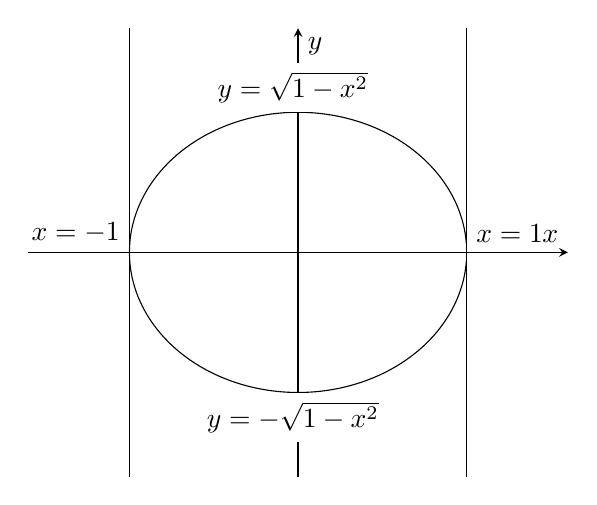
\begin{tikzpicture}
        \begin{axis}[
            axis lines = middle,
            xlabel = $x$,
            ylabel = $y$,
            xmin  = -1.6, xmax = 1.6,
            ymin  = -1.6, ymax = 1.6,
            ticks=none,
            samples=1000,
          ]
            \addplot[domain=-1:1] {sqrt(1 - x^2)} node[midway, above, fill=white] {$y = \sqrt{1 - x^2}$};
            \addplot[domain=-1:1] {-sqrt(1 - x^2)} node[midway, below, fill=white] {$y = -\sqrt{1 - x^2}$};

            \addplot[] ({1}, x) node[midway, anchor=south west] {$x = 1$};
            \addplot[] ({-1}, x) node[midway, anchor=south east] {$x = -1$};
          \end{axis}
      \end{tikzpicture}

      \caption{Bounds of integration on the $xy$-plane}
      \label{fig:bounds_xy_3}
    \end{subfigure}
  \end{figure}

  The bounds for $\rho$ are $0 \le \rho \le 2\cos(\phi)$, the bounds for $\phi$
  are $0 \le \phi \le \frac{\pi}{4}$, and the bounds for $\theta$ are $0 \le
  \theta \le 2\pi$. Converting the integrand to spherical coordinates gives us
  $f(x, y, z) = \rho^2\sin^2(\phi)\cos^2(\theta) +
  \rho^2\sin^2(\phi)\sin^2(\theta) = \rho^2\sin^2(\phi)$.Expanding and
  evaluating the triple integral gives us
  \begin{align*}
    V = \iiint_E f(x, y) \,\dd{V} &= \int_0^{2\pi} \int_0^{\sfrac{\pi}{4}} \int_0^{2\cos(\phi)} \rho^4\sin^3(\phi) \,\dd{\rho} \,\dd{\phi} \,\dd{\theta} \\
                                  &= \int_0^{2\pi} \,\dd{\theta} \cdot \int_0^{\sfrac{\pi}{4}} \sin^3(\phi) \cdot \frac{1}{5}\rho^5\bigg\vert_0^{2\cos(\phi)} \,\dd{\phi} \\
                                  &= 2\pi \cdot \int_0^{\sfrac{\pi}{4}} \frac{32}{5}\sin^3(\phi) \cdot \cos^5(\phi) \,\dd{\phi} \\
                                  &= \frac{64\pi}{5} \cdot \int_0^{\sfrac{\pi}{4}} \cos^5(\phi) (1 - \cos^2(\phi))\sin(\phi) \,\dd{\phi} \\
                                  &= \frac{64\pi}{5} \cdot \left(-\int_{\cos(0)}^{\cos\left(\sfrac{\pi}{4}\right)} u^5 (1 - u^2) \,\dd{\phi}\right) \\
                                  &= \frac{64\pi}{5} \cdot \left(-\int_{1}^{\sfrac{1}{\sqrt{2}}} u^5 - u^7 \,\dd{\phi}\right) \\
                                  &= \frac{64\pi}{5} \cdot \left(-\frac{u^6}{6} + \frac{u^8}{8} \bigg\vert_1^{\sfrac{1}{\sqrt{2}}}\right) \\
                                  &= \frac{64\pi}{5} \cdot \left(\left[-\frac{\sfrac{1}{\sqrt[6]{2}}}{6} + \frac{\sfrac{1}{\sqrt[8]{2}}}{8}\right] - \left[-\frac{1}{6} + \frac{1}{8}\right]\right) \\
                                  &= \frac{64\pi}{5} \cdot \frac{11}{384} = \frac{11\pi}{30}
  .\qedhere\end{align*}
\end{proof}
